Given the curve, 
\begin{align}
    y = \frac{1}{x-3} \label{eq:solutions/1/15/eq:1}\\ 
    \implies xy-3y-1 = 0 \label{eq:solutions/1/15/eq:2}
\end{align}
From \eqref{eq:solutions/1/15/eq:2} we get,  
\begin{align}
    \vec{V} = \frac{1}{2}\myvec{0 & 1 \\ 1 & 0}, \vec{u} = \frac{-3}{2}\myvec{0 \\ 1}, f=-1
\end{align}
Now, 
\begin{align}
    \because \mydet{V} = \mydet{0&\frac{1}{2}\\\frac{1}{2}&0} = \frac{-1}{2}<0
\end{align}

\eqref{eq:solutions/1/15/eq:1} is equation of hyperbola. Now, 
\begin{align}
    \mydet{\lambda\vec{I}-\vec{V}} = \mydet{\lambda & \frac{-1}{2}\\\frac{-1}{2} & \lambda}=0 \\
    \implies \lambda^2-\frac{1}{4} =0
\end{align}
Thus the eigen values are, 
\begin{align}
    \lambda_1 = \frac{1}{2}, \lambda_2 = \frac{-1}{2}
\end{align}
The eigen vector $\vec{p}$ is given by,
\begin{align}
    (\lambda\vec{I}-\vec{V})\vec{p}=0
\end{align}
For $\lambda_1 = \frac{1}{2}$,

\begin{align}
    (\lambda_1 \vec{I}-\vec{V}) = \myvec{\frac{1}{2}&\frac{1}{2}\\\frac{1}{2}&\frac{1}{2}}
    \xleftrightarrow[R_1\xleftarrow{}2R_1]{R_2\xleftarrow{}R_2+R_1}
    \myvec{1&-1\\0&0} \\
    \implies \vec{p_1} = \frac{1}{\sqrt{2}}\myvec{1\\1}
\end{align}
Similarly for $\lambda_2$,
\begin{align}
    (\lambda_2 \vec{I}-\vec{V}) = \myvec{\frac{-1}{2}&\frac{-1}{2}\\\frac{-1}{2}&\frac{-1}{2}}
    \xleftrightarrow[R_1\xleftarrow{}2R_1]{R_2\xleftarrow{}R_-R_1}
    \myvec{1&1\\0&0} \\
    \implies \vec{p_2} = \frac{1}{\sqrt{2}}\myvec{-1\\1}
\end{align}
Now, 
\begin{align}
    \vec{P} = \myvec{\vec{p_1}&\vec{p_2}} = \frac{1}{\sqrt{2}}\myvec{1&-1\\1&1} \\
    \vec{D} = \myvec{\frac{1}{2}&0\\0&\frac{-1}{2}} \\
    \vec{u}^T\vec{V}^{-1}\vec{u}-f=1
\end{align}
$\because  \vec{u}^T\vec{V}^{-1}\vec{u}-f=1>0$, there is no need to swap the axes. The hyperbola parameters are, 
\begin{align}
    \vec{c} = -\vec{V}^{-1}\vec{u} = 3\myvec{1\\0} \\
    \sqrt{\frac{\vec{u}^T\vec{V}^{-1}\vec{u}-f}{\lambda_1}}=\sqrt{2} \\
    \sqrt{\frac{f-\vec{u}^T\vec{V}^{-1}\vec{u}}{\lambda_1}}=\sqrt{2}
\end{align}
with the standard hyperbola becoming, 
\begin{align}
    \frac{x^2}{2}-\frac{y^2}{2}=1
\end{align}
The direction and normal vectors of the tangent with slope $-2$ are given as,
\begin{align}
    \vec{m}=\myvec{1\\-2}, \vec{n}=\myvec{2\\1}
\end{align}
Now considering the equations to find the point of contact, 
\begin{align}
    \vec{q}=\vec{V}^{-1}(k\vec{n}-\vec{u}) \\
    k = \pm \sqrt{\frac{\vec{u}^T\vec{V}^{-1}\vec{u}-f}{\vec{n}^T\vec{V}^{-1}\vec{n}}}
\end{align}
Thus, 
\begin{align}
    \vec{n}^T\vec{V}^{-1}\vec{n}=8 \\
    k= \pm \frac{1}{2\sqrt{2}} \\
    \vec{q_1} = \myvec{\frac{1+3\sqrt{2}}{\sqrt{2}} \\ \sqrt{2}} \\
    \vec{q_2} = \myvec{\frac{-1+3\sqrt{2}}{\sqrt{2}} \\ -\sqrt{2}}
\end{align}
The desired tangents are, 
\begin{align}
    \myvec{2&1} \cbrak{\vec{x}-\myvec{\frac{1+3\sqrt{2}}{\sqrt{2}} \\ \sqrt{2}}} = 0 \\ 
    \implies \myvec{2&1}\vec{x} = 6+2\sqrt{2} \label{eq:solutions/1/15/tangent_1} \\
    \myvec{2&1} \cbrak{\vec{x}-\myvec{\frac{-1+3\sqrt{2}}{\sqrt{2}} \\ -\sqrt{2}}} = 0 \\
    \implies \myvec{2&1}\vec{x} = 6-2\sqrt{2}  \label{eq:solutions/1/15/tangent_2}
\end{align}

Below figure corresponds to the tangents on the hyperbola,  represented by \eqref{eq:solutions/1/15/tangent_1} and \eqref{eq:solutions/1/15/tangent_2} each having slope of $-2$. 
\begin{figure}[h!]
	\centering
	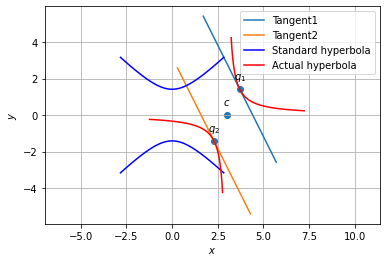
\includegraphics[width=\columnwidth]{./solutions/1/15/assignment_6.png}
	\caption{Tangents to the hyperbola}
	\label{eq:solutions/1/15/fig_1}
\end{figure}



